% Template based upon included TeXworks Basic LaTeX documents article.tex template.

% !TEX TS-program = pdflatex
% !TEX encoding = UTF-8 Unicode

% This is a simple template for a LaTeX document using the "article" class.
% See "book", "report", "letter" for other types of document.

\documentclass[11pt, twocolumn]{article} % use larger type; default would be 10pt

\usepackage[utf8]{inputenc} % set input encoding (not needed with XeLaTeX)

%%% Examples of Article customizations
% These packages are optional, depending whether you want the features they provide.
% See the LaTeX Companion or other references for full information.

%%% PAGE DIMENSIONS
\usepackage{geometry} % to change the page dimensions
\geometry{letterpaper} % or letterpaper (US) or a5paper or....
\geometry{margin=1in} % for example, change the margins to 2 inches all round
% \geometry{landscape} % set up the page for landscape
%   read geometry.pdf for detailed page layout information

\usepackage{graphicx} % support the \includegraphics command and options

% \usepackage[parfill]{parskip} % Activate to begin paragraphs with an empty line rather than an indent

%%% PACKAGES
\usepackage{tikz}
\usetikzlibrary{arrows.meta} % for figures
\usepackage{amsmath}
\usepackage{gensymb}
%\usepackage{unicode-math}

\usepackage{booktabs} % for much better looking tables
\usepackage{array} % for better arrays (eg matrices) in maths
\usepackage{paralist} % very flexible & customisable lists (eg. enumerate/itemize, etc.)
\usepackage{verbatim} % adds environment for commenting out blocks of text & for better verbatim
%\usepackage{subfig} % make it possible to include more than one captioned figure/table in a single float
\usepackage{subcaption}
% These packages are all incorporated in the memoir class to one degree or another...

%%% HEADERS & FOOTERS
\usepackage{lastpage} % page x of y
\usepackage{fancyhdr} % This should be set AFTER setting up the page geometry

\pagestyle{fancy} % options: empty , plain , fancy
%\renewcommand{\headrulewidth}{0pt} % customise the layout...
%\lhead{}\chead{}\rhead{}
%\lfoot{}\cfoot{\thepage\ of \pageref{LastPage}}\rfoot{}

\fancypagestyle{plain}{
  \fancyhf{} 
  \fancyhead[R]{}
  \fancyfoot[C]{\thepage\ of \pageref{LastPage}\\{\scriptsize https://github.com/vwfinley/regarding/blob/main/B/B-001/B-001.pdf}}
  \renewcommand{\headrulewidth}{0pt}
}

\fancyhf{}
  \fancyhead[R]{}
  \fancyfoot[C]{\thepage\ of \pageref{LastPage}}
\renewcommand{\headrulewidth}{0pt}

%%% SECTION TITLE APPEARANCE
\usepackage{sectsty}
\allsectionsfont{\sffamily\mdseries\upshape} % (See the fntguide.pdf for font help)
% (This matches ConTeXt defaults)

%%% ToC (table of contents) APPEARANCE
\usepackage[nottoc,notlof,notlot]{tocbibind} % Put the bibliography in the ToC
\usepackage[titles,subfigure]{tocloft} % Alter the style of the Table of ContentsT
\renewcommand{\cftsecfont}{\rmfamily\mdseries\upshape}
\renewcommand{\cftsecpagefont}{\rmfamily\mdseries\upshape} % No bold!

% Package for boxes around aligned equations
\usepackage{empheq}
\newcommand*\widefbox[1]{\fbox{\hspace{2em}#1\hspace{2em}}}

% Packages for complex tables
\usepackage{multirow}
\usepackage{makecell}

% Package for long multilined equations
%\usepackage{mathtools}
\usepackage{breqn}

% For boxed multiline equations
\usepackage{empheq}

% SVG files
\usepackage[inkscapeformat=pdf]{svg}

% Packages for Blockquotes
\usepackage{setspace} % for \onehalfspacing and \singlespacing macros
\onehalfspacing 
\usepackage{etoolbox}
\AtBeginEnvironment{quote}{\par\singlespacing\small}

% Endnotes package
\usepackage{endnotes}
\renewcommand{\notesname}{Endnotes}

% Packages for figures
%\usepackage{graphicx}
%\usepackage{caption}
%\usepackage{subcaption}

%%% END Article customizations

%%% The "real" document content comes below...

\title{B-001\\Regarding NMRA RP-25}
\author{Vincent W. Finley\thanks{\copyright 2022: Bear, DE, USA: CC BY 4.0 license\\https://creativecommons.org/licenses/by/4.0/legalcode}}
\date{November 2022} % Activate to display a given date or no date (if empty),
         % otherwise the current date is printed 

\begin{document}
\maketitle

Study of the Tangent Ogive has useful applicaton in Engineering, especially to ballistics and aeronautics.
Previous investigation described how the Tangent Ogive may be defined by inscribing the ogive upon a circle.  
It also described relationship of the ogive parts.

While basic ogive analysis is indispensable, further exploraration of the Tangnet Ogive is desired.
What are its properties?  
More pertinently, how can it be used in other mathmatical solutions?
\section{Introduction}
While concise, the RP-25 document can be perplexing.
Discussion of the wheel-contour construction process is absent.
Locations of circle centers are omitted.
Calculations of circle radius values are conspicuously missing.
Important information is implied or excluded.

Understanding 1960s technology aids in understanding the RP-25 document.
Most of the omitted information may have been obvious to technical people, of the early 1960s, when RP-25 was written.
Technology was analog for most of the population.
Systems were designed and drawn with simple drafting tools.
Secondary school graduates would have been well-trained in constructive geometry.
Mechanical design was mainly accomplished by applying Euclidean techniques, rather than algebraic or trigonometric calculation.
Calculations were performed by hand, when required, or perhaps with a sliderule.

Prior to inexpensive digital personal computers and computer aided drawing (CAD), most design work involved analog drafting tools.
Digital calculators may have substituted later for sliderules, however, designs and drawings were still analog.
Although the current RP-25 document is typeset as a *.pdf document, the design is still vintage 1960s analog.



\section{Problem}
How does one draw the RP-25 wheel contour?
Don't think in terms of wheel treads and flanges!
The trick to solving this problem is framing it mathematically.

Reduce the problem to its most fundamental mathematic idea.
Simplify!
The problem of drawing the RP-25 contour is really just a problem of drawing three circles in the correct locations!

\paragraph{Given:}
\begin{itemize}
\item Three circles: $C1$, $C2$, $C3$; whose radii are: $R1$, $R2$, $R3$; respectively...
\item with $0 < R1 < R2 = R3$
\end{itemize}

\paragraph{Find:}
\begin{enumerate}
\item Circle center locations: $P1$, $P2$ and $P3$; such that:
\item $C1$ is tangent to the horizontal line passing some distance $P$ above the origin
\item with, $C1$ and $C2$ mutually tangent to each other, at the origin
\item and with, $C2$ and $C3$ intersecting at some location: $P - D'$ below, and $T/2$ to right of; the origin.
\end{enumerate}

%\section{Context}
While concise, the RP-25 document can be perplexing.
Discusson of the wheel-contour construction process is absent.
Locations of circle centers are omitted.
Calculation of circle radius values is conspicuously missing.
Important information is implied or leftout.

Understanding 1960s technology aids in understanding the RP-25 document.
Most of the omitted information may have been obvious to technical people, of the early 1960s, when RP-25 was written.
Technology was analog for most of the population.
Systems were designed and drawn with simple drafting tools.
Secondary school graduates would have been well-trained in constructive geometry.
Mechanical design was mainly accomplished by application of Euclidean constructive geometry, rather than algebraic or trigonometric calculation.
Calculations were performed by hand, when required, or perhaps with a sliderule.

Prior to inexpensive digital personal computers and computer aided drawing (CAD), most designwork involved analog drafting tools.
Digial calculators may have substituted later for sliderules, however, designs and drawings were still analog.
Although the current RP-25 (July 2009 version) document is typeset as a *.pdf document, the design is still of the 1960s analog heritage.





% VWF NOTE: Add drawings to theorems
% VWF NOTE: Add discussion of gage point as origin.


\section{Geometric Theorems}
Three helpful plane geometric theorems are declared here.
They will be used throughout the solution.
They are paraphrased from their original sources and are stated here without proof.
A curious reader will find those sources referenced in the endnotes section.


% VWF NOTE: Arcs or chords?  Any two points?  Or points such that they intersect?
\paragraph{Theorem 1: Circle Center}
\begin{quote}
The center of a circle (or arc), of radius $r$, can be found by 
constructing arcs of radius $r$ centered about any two points on the circle.
The circle's center shall coincide with intersection
of constructed arcs.\endnote{Machinery's Handbook 25th Edition,
Robert E. Green, Editor
Copyright 1996,
Industrial Press Inc.,
ISBN 0-8311-2424-5,
Page 51, 
Paraphrased from first construction on page}
%\subsection{Theorem 2: Mutually tangent circles}
%\begin{quote}
%If two circles (or arcs) are tangent to each other externally or internally, the line of centers
%passes through the point of tangency.
%\endnote{
%Practical Shop Mathematics,
%Volume 1 Elementary, 
%John H. Wolfe and Everett R. Phelps, Ph.D.
%Copyright 1935 \& 1939,
%McGraw-Hill Book Company, Inc.,
%Page 144,
%Proposition 43}
%\end{quote}
\end{quote}
\paragraph{Theorem 2: Mutually tangent circles}
\begin{quote}
If two circles contact each other at a single point, the centers and 
the contact point are collinear.\endnote{
The First Six Books of the Elements of Euclid, 
3rd Edition,
John Casey and Euclid,
1885,
Hodges, Figgis \& Co., Dublin,
Longmans, Green \& Co., London,
Page 78,
Observation: Propositions XI, XII
https://www.gutenberg.org/files/21076/21076-pdf.pdf
}
\end{quote}
\paragraph{Theorem 3: Bisection of isosceles triangle}
\begin{quote}
The bisector of the vertical angle of an isosceles triangle is perpendicular to the base 
and bisects the base.\endnote{
Practical Shop Mathematics,
Volume 1 Elementary, 
John H. Wolfe and Everett R. Phelps, Ph.D.
Copyright 1935 \& 1939,
McGraw-Hill Book Company, Inc.,
Page 105,
Corollary 1 to Proposition 19}
\end{quote}
\section{Solution}
\subsection{Sub1}
Todo: Write me.


%\begin{figure}[htbp]
%  \centering
%  \includesvg{drawing.svg}
%  \caption{svg image}
%\end{figure}

\begin{figure}[ht!]
\centering

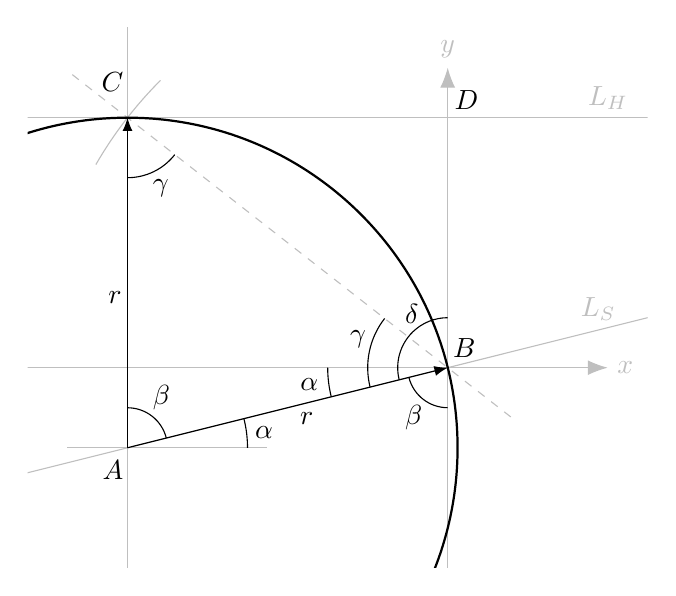
\begin{tikzpicture}[x=1in, y=1in]
	\begin{scope}[xscale=.10, yscale=.10]	

%		\coordinate (origin) at (0,0);
%		\coordinate (P1) at (-0.0134, -0.0040);
%		\coordinate (P2) at (.0214, .0064);
%		\coordinate (P3) at (0.0086, 0.0064);
%		\coordinate (Pf) at (0.015, -0.015);
%		\coordinate (Pb) at (0.030, 0);
%		\coordinate (Pm) at (0.0075, -0.0075);		

		\clip (-21, -10) rectangle (10, 17);

		% axes
		\draw[lightgray, -{Latex[scale=1.5]}] (0, -30.0) -- (0, 15.0)  node [above] {$y$};	
		\draw[lightgray, -{Latex[scale=1.5]}] (-40.0, 0) -- (8.0, 0)  node [right] {$x$};		

		% vertical
		\draw[lightgray] (-16.0097, -35) -- (-16.0097, 35); % left

		% horizontal
		\draw[lightgray] (-50, 12.5) -- (90, 12.5) node[shift={(179.3 : 8.2)}]{$L_H$}; % L_H
		\draw[lightgray] (-19.0097, -4.0024) -- (-9.0097, -4.0024);	 % R center mark

		% sloped
		\draw[lightgray] (194.04 : 58) -- (14.04 : 98) node[shift={(-166.6 : 9.0)}]{$L_S$}; % L_S

		% bisector
		\draw[lightgray, dashed] (142.02 : -4) -- (142.02 : 24); % dashed line
		\draw[lightgray] ([shift=(135 :  20.3116)] 0, 0)  arc (135 : 150 : 20.3116); % mark

		% angle labels
		\draw[black] ([shift=(180 : 6)] 0, 0)  arc (180 : 194.04 : 6) node[shift={(-0.11, 0.06)}]{$\alpha$} ; % alpha
		\draw[black] ([shift=(194.04 : 2)] 0, 0)  arc (194.04 : 270 : 2) node[shift={(-0.17, -0.05)}]{$\beta$}; % beta
		\draw[black] ([shift=(142.02 : 4)] 0, 0)  arc (142.02 : 194.04 : 4) node[shift={(-0.06, 0.24)}]{$\gamma$}; % gamma

\draw[black] ([shift=(194.04 : 2.5)] 0, 0)  arc (194.04 : 90 : 2.5) node[shift={(-0.18, 0.02)}]{$\delta$}; % gamma

		\draw[black] ([shift=(0 : 6)] 194.04 : 16.5024)  arc (0 : 14.04 : 6) node[shift={(0.1, -0.07)}]{$\alpha$}; % alpha
		\draw[black] ([shift=(14.04 : 2)] 194.04 : 16.5024)  arc (14.04 : 90 : 2) node[shift={(0.17, 0.05)}]{$\beta$}; % beta		
		\draw[black] ([shift=(142.02 : 20.3116)] 270 : 3)  arc (270 : 322.02 : 3) node[shift={(-0.07, -0.17)}]{$\gamma$}; % gamma


		% locate arc
%		\draw[black] ([shift=(-40 : 16.5024)] 194.04 : 16.5024) arc (-40  : 105 : 16.5024); % The arc
		\draw[black, thick] (194.04 : 16.5024) circle (16.5024); % The arc
		
		% radius lines
		\draw[black, -{Latex[scale=1.0]}] (194.04 : 16.5024) -- +(90 : 16.5024) node[shift={(-94 : 0.9)}]{$r$};
		\draw[black, -{Latex[scale=1.0]}] (194.04 : 16.5024) -- +(14.04 : 16.5024) node[shift={(200 : 0.75)}]{$r$};

		% Labels
		\draw[black] (197 : 17.5)  node{$A$};
		\draw[black] (50 : 1.3)  node{$B$};
		\draw[black] ((139.6 : 22)  node{$C$};
\draw[black] ((86 : 13.4)  node{$D$};

	\end{scope}
		





\end{tikzpicture}
\caption{Tangent Ogive Alternate Construction}
\label{fig:fig_a}
\end{figure}



\begin{flushright}   
Q.E.D.
\end{flushright}
\section{Example}

\paragraph{Given:}
\begin{itemize}
\item Two circles $A$ and $B$ whose radii are $r_A = r_B = 3.0$ units,
\item \emph{and} circle centers $C_A$ and $C_B$ separated by a distance of 9.0 units.
\end{itemize}

\paragraph{Find:}
\begin{itemize}
\item Which solution case and tangent class best matches the given arrangement.
\item All tangent lines and any point of intersection.
\item Any angle of intersection between tangent lines.
\end{itemize}

\paragraph{Steps:}
\begin{enumerate}
\item
Let: 
\begin{align*}
	x_A &= 9.0 \\
	r_A &= 3.0 \\
	r_B &= 3.0
\end{align*}

\item
From the solution section, use the inequality for case 9:
\begin{equation*}
	x_A > 2  \cdot r_A
\end{equation*}

\item
Plug in values for $r_A$,
\begin{equation*}
	9.0 > 2  \cdot 3.0
\end{equation*}
\begin{equation*}
	9.0 > 6.0
\end{equation*}

\item
Since $x_A = 9.0$ is greater than $6.0$, $x_A$ satisfies the inequality for case 9.  Therefore the relationship
between circles $A$ and $B$ are classified by case 9.

\item
From Table \ref{table:tab_tangents} it is found that case 9 will have two Outer tangents and two Inner tangents.

\item
Outer class:

The upper an lower horizontal tangent lines will lie a distance $r_A = 3.0$ above and below the x-axis.  Tangents will be parallel 
and will not intersect.

\item
Inner class:

Substituting in $9.0$ for $x_{A'}$ into equation \ref{eq:IResult} yields:
\begin{align*}
I &= \left(\frac{x_{A'}}{2}, 0\right)\\
I &= \left(\frac{9.0}{2}, 0\right)
\end{align*}
\begin{equation*}
\boxed
{
I = (4.5, 0)
}
\end{equation*}


Substituting for $x_{A'}$  and $r_A$ into equation \ref{eq:thetaarcsin} yields:
\begin{align*}
\theta &= 2 \cdot \arcsin{\left( \frac{2 \cdot r_A}{x_{A'}}  \right)}\\
\theta &= 2 \cdot \arcsin{\left( \frac{2 \cdot 3.0}{9.0}  \right)}\\
\theta &= 2 \cdot \arcsin{\left( \frac{6.0}{9.0}  \right)}\\
\theta &= 1.45946 \hspace{1 mm} rads
\end{align*}
\begin{equation*}
\boxed
{
\theta = 83.62^{\circ}
}
\end{equation*}

\end{enumerate}
\theendnotes
\end{document}
